\section{Implementation of Asynchronous Read}
\subsection{XDR}
We generated the request and response structures for our \textsc{asynchronous read} using the eXternal Data Representation (XDR) \cite{XDR}. XDR is a standard data serialization format. XDR allows the data to be transferred seamlessly between different kinds of systems. Let us now look at each of these structures in detail.

\begin{lstlisting}
struct ASYNC_READ4args{
	uint64_t  reqid; 
	stateid4  stateid; 
	offset4	  offset; 
	count4	  count;
	uint32_t  timeout; 
};
\end{lstlisting}

\noindent\textit{ASYNC\_READ4args} : The client sends these argument structure as part of the initial request to the server. Detailed explanation of the arguments in \textit{ASYNC\_READ4args} will follow. 
\hfill \break \newline
\noindent\textit{reqid} : \textit{reqid} is a 64 bit integer, generated by the client. This is generated based on the requested \textit{filehandle}, processid/threadid and current\_timestamp and will uniquely identify every request. The server passes the same \textit{reqid} to the client as part of the callback along with the requested file data. The client process/thread then uses this  \textit{reqid} to uniquely identify the request among multiple requests that it might have triggered to the server. Note that \textit{reqid} is opaque to the server.
\hfill \break \newline
\noindent\textit{stateid} : \textit{stateid} is a 128-bit quantity returned by a server in the initial open request. It uniquely defines the \textit{open} and locking state provided by the server for a specific open or lock owner for a specific file. We are using \textit{stateid} on the server side to check the client share/delegation access on the requested file. 
\hfill \break \newline
\noindent\textit{offset} : \textit{offset} is offset from the start of the file at which the read has to start in the file. 
\hfill \break \newline
\noindent\textit{count}: Number of bytes to read from the requested file.
\hfill \break \newline
\noindent\textit{timeout}: \textit{timeout} is a configurable field in milliseconds. This field specifies the maximum time that the server can take to respond with a callback once it receives the asynchronous read request. This field is important for the client to identify server crashes and any network outages. If the client doesn't receive the response in the specified time, it treats the request as a failure and resends the request.     
\hfill \break \newline
\noindent On receiving the request from the client, the server performs the initial checks. Then the server responds with \textsc{ASYNC\_READ4res} to the client. Now we will explain the status passed as part of \textsc{ASYNC\_READ4res} to the client.  

\begin{lstlisting}
struct ASYNC_READ4res{
	nfsstat4	  status;
};
\end{lstlisting}

\textit{status} : Indicates the \textit{status} corresponding to initial permission checks on the requested file.
On receiving the \textsc{asynchronous read} request on the server side, we are checking the client's share/delegation on the requested file. On success we will return \textsc{nfs4\_ok}.  If the checks fail, we are returning appropriate error status.
\hfill \break \newline
\noindent Let us now understand the structure used by the server when making a callback to the client. The server passes \textit{CB\_ASYNC\_READ4args} as part of the request to the client. We will now look at each of the arguments in detail. 
\begin{lstlisting}
union CB_ASYNC_READ4args 
	switch(nfsstat4 status){
	case NFS4_OK:
	 CB_ASYNC_READ4argsok argok4;
 	default:
		void;
};
\end{lstlisting}

\noindent The first argument in the callback request to the client is the \textit{status}. If the data is fetched successfully from the local file system, the \textit{status} will be \textsc{nfs4\_ok}. In case of an error, an appropriate error \textit{status} will be sent to the client. If the data is fetched successfully, a second argument of type \textit{CB\_ASYNC\_READ4argsok} will also be passed in the callback to the client. Otherwise, only \textit{status} will be passed. A detailed explanation of each of the fields in \textit{CB\_ASYNC\_READ4argsok} will follow.

\begin{lstlisting}
struct CB_ASYNC_READ4argsok{
	uint64_t	 reqid;
	bool		 eof;
	opaque	data<>;
};
\end{lstlisting}

\noindent\textit{reqid}: The \textit{reqid} received by the server from the client during the initial asynchronous read request. This is used by the client to identify the owner of the request.
\hfill \break \newline
\noindent\textit{eof} : A boolean value indicating if the end of the file has been reached.
\hfill \break \newline
\noindent\textit{data} : Requested file \textit{data}.
\hfill \break \newline
\noindent On receiving the callback request from the server, client forwards the data to the respective owner based on the \textit{reqid}. Then the client responds with \textsc{CB\_ASYNC\_READ4res} to the server.
 
\begin{lstlisting}
struct CB_ASYNC_READ4res{
	nfsstat4	 status;
};
\end{lstlisting}

\noindent\textit{status} : Indicates the asynchronous read callback \textit{status} from the client. On success, status will be \textsc{nfs4\_ok} else the corresponding error message will be passed to the server.


We will now discuss the existing implementation of \textsc{nfs\_read} in NFS-Ganesha. Understanding \textsc{nfs\_read} is important as we have reused the design of \textsc{nfs\_read} for performing actual read during callback in asynchronous read operation.


\begin{figure*}
\centering
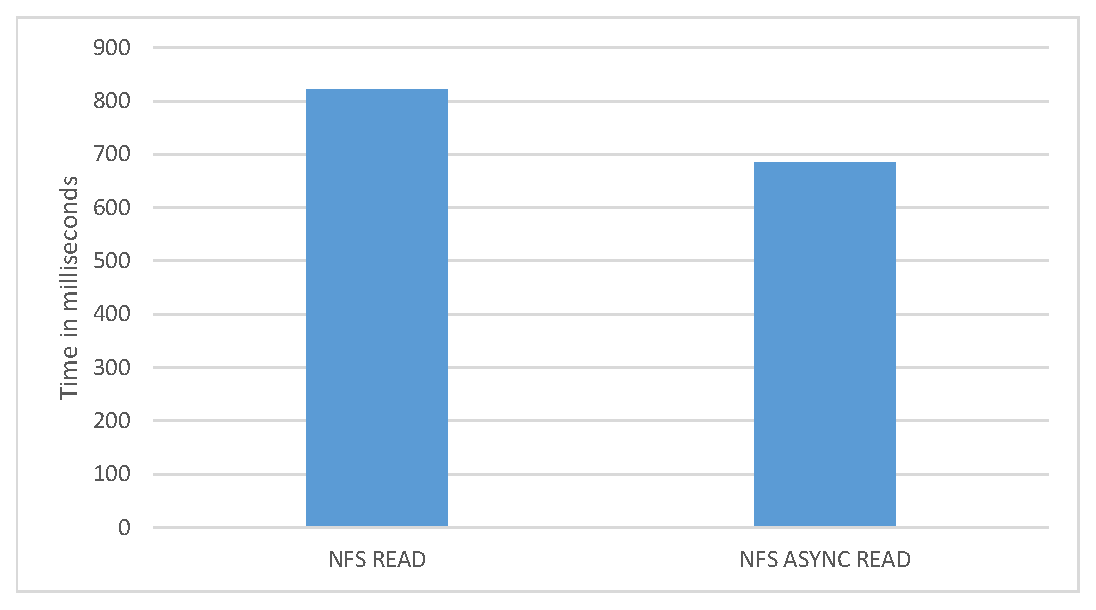
\includegraphics[scale=1.0]{figures/InterstingObservation.eps}
\caption{Intersting observation incase of two consequtive requests on a hard disk}
\label{fig:InterstingObservation}
\end{figure*}

\subsection{Implementation of NFS READ in Pynfs Client}
 
From \textsc{NFSv4.0} and above, all the NFS operation are performed using compound requests. A compound request can consist of multiple requests. The server will process the compound procedure by evaluating each of the operations within the compound procedure in order. For a normal read, the Pynfs client prepares a \textsc{nfs4\_compound} request consisting of two operations. The first operation is the \textsc{putfh}. \textsc{putfh} is used as the first operator in an \textsc{nfs request} to set the context for following operations. This operation replaces the current \textit{filehandle} with the \textit{filehandle} of the file to be read. It is then followed by an actual \textsc{read} operation. The \textsc{read} operation reads data from the \textsc{regular file} identified by the current \textit{filehandle}. Once the NFS clients sends the request, it waits for a configurable amount of time. If it does not receive the response in the stipulated time, an RPC timeout error will be signalled. Once the client receives the response, several validation checks are performed to identify the failures.



\subsection{Implementation of NFS READ in Pynfs Server}
Pynfs server on receiving the READ request, spawns a thread to process the request. The server first performs validation on the \textit{stateid}. If mandatory file locking is \textsc{on} for the file, and if the region corresponding to the data to be read from file is write locked by an owner not associated with the \textit{stateid}, the server will return the \textsc{nfs4err\_locked} error. If all the tests are passed, the server then does a read on the file identified by the current \textit{filehandle}. The file is read from the offset indicated in the request.  If the read ended at the end-of-file, \textit{eof} is returned as  \textsc{true}. Otherwise it is \textsc{false}. The response is then encoded in XDR format and is sent back to the client.
	
\subsection{Implementation NFS READ in NFS-Ganesha}

 The request processing in NFS-Ganesha is done by pthreads. Figure~\ref{fig:NFSReadArch} depicts the architecture diagram of \textsc{nfs\_read} in NFS-Ganesha. The dispatcher thread will listen for incoming \textsc{nfs request} but will not decode them. It will choose the least busy worker and add the request to its lists of requests to process. Duplicate request management is also done by the dispatcher thread. One of the worker thread will then dequeue the request from the worker queue and process it. The worker threads do most of the job. These threads are very core to the NFS processing in NFS-Ganesha. The processing of a read request involves validating the client access on the requested file. On success, the worker thread will decode it and use Cache Inode API and File Content API calls to perform the read required for this request. Once the server has retrieved the data successfully from the underlying file system, it will then send the response back to the client with the requested data.
  

\subsection{Implementation of NFS Asynchronous Read in Pynfs Client}
 
The client side operations for asynchronous read are similar to that of a normal read. Once the request is sent, the client keeps track of them based on their \textit{reqid} and \textit{stateid}. If the client doesnot hear back from the server in the \textit{timeout} specified in the request, the client times out and resends the request. The client uses both \textit{reqid} and \textit{stateid} to keep track of the requests that are sent to the server.  Here \textit{reqid} is essential because the same file owner might have triggered multiple request on the same file.  
  
\subsection{Implementation of NFS Asynchronous Read in Pynfs Server}
 \textsc{nfs async read} implementation is mostly similar to that of a \textsc{nfs read} operation. On receiving the request the server performs validation on the \textit{stateid}. If mandatory file locking is \textsc{on} for the file, and if the region corresponding to the data to be read from file is write locked by an owner not associated with the \textit{stateid}, the server will return the \textsc{nfs4err\_locked} error. The client should try to get the appropriate read record lock via the \textsc{lock} operation before re-attempting the \textsc{read}. Otherwise, if the file is free to read, the server will spawn a second thread to process the read request. The first thread that received the request will reply back with a \textsc{nfs4\_ok} status to the client. The second thread then does a read on the file identified by the current \textit{filehandle}. Once it fetches the required data to serve the request, it then triggers a callback request to the client with the data. The server also keeps track of the all the \textit{reqid}s for which an \textsc{nfs callback} is yet to be sent.
 
    
\subsection{Implementation NFS Asynchronous Read in NFS-Ganesha}  

 Figure~\ref{fig:NFSAsyncReadArch} depicts the architecture diagram of \textsc{nfs\_asyncread} in NFS-Ganesha. The dispatcher thread will listen for incoming NFS requests but will not decode them. It will choose the least busy worker and add the request to its lists of requests to process. The worker thread then performs validation on the \textit{stateid}. If  the checks succeed, an \textsc{nfs4\_callback} request is enqueued back into the list of requests to be processed.  This involves preparing a new \textsc{nfs request} for the callback and then en-queuing the request into the worker queue. After en-queuing the callback, the worker thread responds with an \textsc{nfs4\_ok} back to the client. On receiving the initial response, client is freed from the blocking call and can perform further tasks. Now on the server side, a least busy worker will dequeue this new request and process it. This worker thread will perform the actual file system read/cache read depending on the presence of data. After reading the data, \textsc{cb\_async\_read} request is sent to the client via the callback channel. The worker thread which has performed the actual read dispatches the callback request to the client. 
 
\begin{figure*}
\centering

\includegraphics[scale=0.6]{figures/performancesequence.eps}
\caption{Throughput for NFS Asynchronous read and normal NFs read on a flash storage}
\label{fig:performancesequence}
\end{figure*}




 
 
 








